\documentclass{article}
\usepackage[utf8]{inputenc}
\usepackage[T1]{fontenc}

\usepackage{fullpage}

\usepackage{tikz}
%\usetikzlibrary{calc,arrows,shapes,backgrounds,patterns,fit,decorations,decorations.pathmorphing}

\usepackage[shadow,colorinlistoftodos,textwidth=2.5cm]{todonotes}
\usepackage[final,colorlinks,hyperindex,unicode=true,pdftitle=SPAdes Manual]{hyperref}
\usepackage{url}
\usepackage{booktabs}

\def\spades{SPAdes}
\def\bh{BayesHammer}
\def\ecoli{\it E.~coli}

\usepackage{textcomp}
\usepackage{listings}
\definecolor{light-gray}{gray}{0.92}
\lstset{
  upquote=true,
  columns=fullflexible,
  basicstyle=\ttfamily,
  framerule=0pt,
  frame=single,
  backgroundcolor=\color{light-gray},
  literate={*}{{\char42}}1
           {-}{{\char45}}1
}

%\usepackage[space=true]{accsupp}
%% requires the latest version of package accsupp
%\newcommand{\copyablespace}{
%    \BeginAccSupp{method=hex,unicode,ActualText=00A0}
%\ %
%    \EndAccSupp{}
%}


%\newenvironment{mycode}
%  {\begin{lstlisting}}
%  {\end{lstlisting}}

\begin{document}
\title{{\spades} 2.0.0 Manual\\{\small 
  Revision: \today}}
\date{}
\maketitle

{\spades} stands for St.~Petersburg genome assembler.
It is intended for both single cell MDA and standard (multicell) 
assemblies. 
%{\spades} comes with error correction tool called BayesHammer. 
This manual will help you to install and run
{\spades}. The latest version of the manual can be downloaded at \url{http://bioinf.spbau.ru/spades}.


\renewcommand{\contentsname}{}
\tableofcontents

%\pagebreak

%\listoftodos

\pagebreak

\section{General setting}
\subsection{Notation}
{\spades} works with single and forward-reverse paired end reads.
The following picture explains the notions of 
read length, distance, gap, and insert size
for forward-reverse paired end reads.

\begin{center}
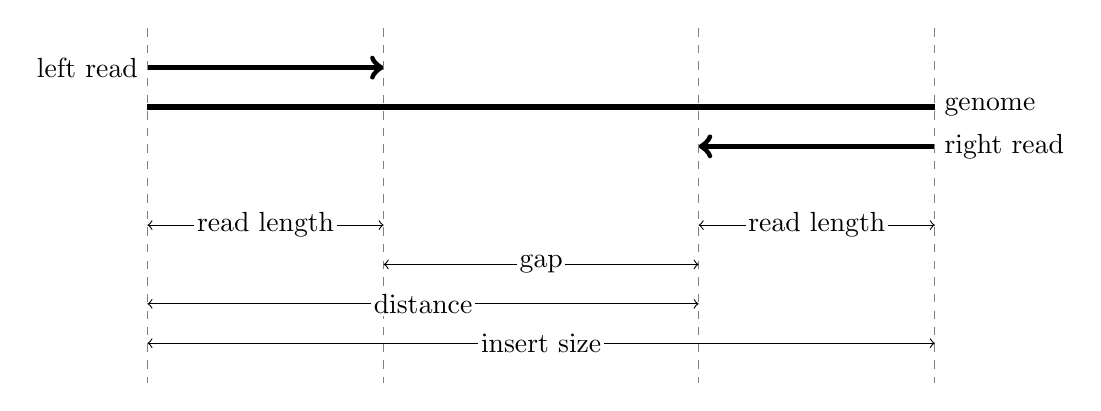
\begin{tikzpicture}
%\draw[help lines] (0,-3) grid (10,3);
\draw[line width=2pt] (0,2) -- (10,2);
\draw[line width=2pt,->] (0,2.5) -- (3,2.5);
\draw[line width=2pt,->] (10,1.5) -- (7,1.5);

\node[rectangle,anchor=east] at (0,2.5) {left read};
\node[rectangle,anchor=west] at (10,2) {genome};
\node[rectangle,anchor=west] at (10,1.5) {right read};

\foreach \x in {0, 3, 7, 10}
  \draw[dashed,gray] (\x,3) -- (\x,-1.5);

\foreach \f/\s/\y/\t in {0/3/0.5/read length, 7/10/0.5/read length, 3/7/0/gap, 0/7/-0.5/distance, 0/10/-1/insert size}
\path[<->,draw] (\f,\y) -- node[fill=white,inner sep=1pt,rectangle] {\t} (\s,\y);
\end{tikzpicture}
\end{center}

\subsection{Config files and commands}
Config files and commands are given in gray boxes. 
In config files, the part of a line starting with a semicolon is a comment.

Note that the text can be copy-pasted directly from this document
and that all the links and all the colored text in the manual are clickable.


\section{Requirements}
\subsection{Operating System}
{\spades} requires a 64-bit Linux system.
You need to have root privileges in order to install {\spades}.

\subsection{RAM}
Assembling our test multi-cell {\ecoli} dataset 
by {\spades} uses about 700~Mb peak memory, and single cell
{\ecoli} dataset uses 6~Gb peak memory. 
Correcting errors in these datasets requires about 70~Gb of RAM.
These datasets can be found at \url{http://spades.bioinf.spbau.ru/spades_test_datasets}.

\section{Installing {\spades}}
\subsection{Installing Debian package (for Debian, Mint, Ubuntu, etc)}
First, add the repository containing {\spades} by inserting the following line
to the file {\tt /etc/apt/sources.list}
\begin{lstlisting}
deb http://debian.bioinf.spbau.ru /
\end{lstlisting}
and update the package list by typing
\begin{lstlisting}
sudo apt-get update
\end{lstlisting}
After that, {\spades} can be installed just by typing
\begin{lstlisting}
sudo apt-get install spades
\end{lstlisting}

\subsection{Installing RPM package (for CentOS, Fedora, Mandriva, Red Hat, SUSE, etc)}
\todo[inline]{to be written; waiting for Yasha}

\subsection{Testing your installation}
To check your installation type
\begin{lstlisting}
spades.py
\end{lstlisting}
This runs {\spades} on a toy dataset (first 1,000 bp of {\ecoli}) that {\spades} comes with. If the installation was successfull you will see the following lines in the end of the run.
\begin{lstlisting}
All the resulting information can be found here:
/usr/share/spades/output/ECOLI_1K/spades_04.11_08.26.04
 * Resulting contigs are called ECOLI_1K.fasta
 * Assessment of their quality is in
  /usr/share/spades/output/ECOLI_1K/spades_04.11_08.26.04/quality_results/

Thank you for using SPAdes!

===== Assembling finished. Log can be found here:
/usr/share/spades/output/ECOLI_1K/spades_04.11_08.26.04/assembly.log


===== SPAdes pipeline finished
\end{lstlisting}\todo{update}

%\section{Input format}
%{\spades} accepts single reads as well as forward-reverse paired end reads
%in FASTA and FASTQ format. The number of files with single reads may be arbitrary while paired end %reads should be organized into one or two files. In a single file, each left read should be %followed by its mate right read. In case of two files, the first file should contain all left %reads while the second one should contain all the corresponding right reads in exactly the same %order. All the files may be compressed.

%Note that currently {\spades} works with only one library.

\section{Running {\spades}}\label{sec:running}
To run {\spades} type
\begin{lstlisting}
./spades.py <config.info>
\end{lstlisting}
%Note that the script requires {\tt python} version~2.6.
%If your default {\tt python} version is lower, type
%\begin{lstlisting}
%python26 ./spades.py <config.info>
%\end{lstlisting}
By default (i.e., if no config file is given) {\spades} uses the file {\tt spades\_config.info}. 
Below we first give an example of a config file
and then explain its contents in detail.

\begin{lstlisting}													
; all paths are relative to the working directory but you can also use 
; $cfg variable to set paths relative to this config

project_name        ECOLI_1K                          ; optional. Name of this config file is used if not specified
output_dir          ./spades_output
output_to_console   true                              ; optional. Default is true

dataset
{
    paired_reads $cfg/test_dataset/ecoli_1K_1.fq.gz $cfg/test_dataset/ecoli_1K_2.fq.gz
    single_reads ; optional
    single_cell         false
}

error_correction
{
    tmp_dir                                           ; optional. <output_dir>/corrected/tmp is used if not specified
    qvoffset                                          ; optional. Either 33 or 64
    max_iterations      4
    max_threads         20
    max_memory          50 ; in GB
    gzip_output         true
}

assembly
{
    iterative_K         21 33 55
    paired_mode         true
    generate_sam_files  true                          ; optional. Default is false
}

quality_assessment      ; optional. If section exists (even if it has no lines) than spades.py evaluates quality of the final contigs
{
    reference           $cfg/test_dataset/E.coli/MG1655-K12.first1K.fasta.gz ; optional
    genes               $cfg/test_dataset/E.coli/genes.first1K.txt           ; optional
    operons             $cfg/test_dataset/E.coli/operons.first1K.txt         ; optional
}
\end{lstlisting}

The first thing to notice is that besides of global variables the config file contains three sections. The first one ({\tt error\_correction}) is responsibe for correcting errors in the input reads.
Note that for an accurate assembly it is important to use this stage, especially
for single-cell datasets.
The second one section ({\tt assembly}) 
containg assembly settings.
The last section ({\tt quality\_assessment})
is needed for estimating the quality of the resulting assembly.
To run only some of these three stages just remove (or comment) the unnecessary stages.

%If both sections are present {\spades} first corrects errors in the reads specified by {\tt %input\_reads} and then assembles the resulting reads. Also, the dataset file
%with the resulting reads is created in the folder specified by {\tt output\_dir}.

\subsection{Global settings}
\begin{description}
\item[{\tt project\_name}] specifies the name of the project. It is recommended to set a meaningful name for each separate project. This makes easier to find the results in the output folder.
\item[{\tt output\_dir}] specifies the output folder.
\item[{\tt output\_to\_console}] flag controls outputting log messages to the console.
\end{description}

\subsection{Dataset settings}
{\spades} accepts single reads as well as forward-reverse paired end reads
in FASTA and FASTQ format. All the files may be compressed. Currently {\spades} works with only one library.

\begin{description}
\item[{\tt paired\_reads}] specifies input paired end reads organized into one or two files.
In a single file, each left read should be followed by its mate right read. In case of two files, the first file should contain all left reads while the second one should contain all the corresponding right reads in exactly the same order (two files should be separated by a space).
\item[{\tt single\_reads}] specifies reads without pairs. You can specify any number of
files with single reads.
\item[{\tt single\_cell}] flag is set if input data was obtained with mda (single cell) technology.
\end{description}

\subsection{Error correction settings}
\todo[inline]{to be written}

\subsection{Assembly settings}\label{subsec:assembly}
\begin{description}
\item[{\tt iterative\_K}] specifies one or more odd values for $k$-mer (vertex) sizes.  Informally, smaller values of $k$ make the graph more connected, but at the same time more tangled, while higher values of $k$ may defragment the graph, but allow to resolve short repeats. The typical value for this variable is {\tt 21 33 55}. See the paper (\cite{main}) for more details.  Note that in the configuration file, $K$ is the size of a vertex, while in the paper, $K$ is the size of an edge (one higher).

\item[{\tt paired\_mode}] turns on/off the repeat resolver.

\item[{\tt dataset}] is the name of the file specifying the dataset to be assembled
(see section~\ref{sec:datasets}). Note that this field is not needed (and not used)
if the {\tt bh} section is present as in this case the dataset file is created automatically.

\item[{\tt measure\_quality}] flag: if set to true, the quality estimation tool will be called after the assembly is performed.  The tool computes metrics such as N50, genome coverage, number of misassemblies, etc.
\end{description}

\subsection{Quality assesment settings}
If this section is present in the config file then
{\spades} computes statistics on various metrics (like N50) of the resulting contigs.
\todo[inline]{to be written}


\section{Understanding the output}
Results can be found in the folder specified by {\tt output\_dir}.
The specific directories containing corrected reads, assembly, and quality estimate are given
at the end of the log.

\section{Postprocessing}

\subsection{Correcting errors in the resulting contigs}
While {\spades} produces accurate assemblies, 
we recommend running SEQuel~\cite{sequel} after {\spades} to further reduce the number of small errors (single nucleotide substitutions and small indels). SEQuel is available at
\url{http://bix.ucsd.edu/SEQuel/}. Note that one can set the flag {\tt generate\_sam} to {\spades}
(see subsection~\ref{subsec:assembly}) to generate a SAM-file showing how the 


\subsection{Scaffolding}
The current version of {\spades} does not have a scaffolding stage.
One can use a separate scaffolder such as Opera~\cite{opera}.
It is available at \url{http://sourceforge.net/projects/operasf/}.

\section{Bug reports}
Bug reports should be sent to \url{spades.support@bioinf.spbau.ru}.


\bibliographystyle{plain}
\bibliography{manualbib}


\end{document}
